The idea behind the data structure used is that, by the user only having one vote for each played track, the user is only given one reference to a track which is a vote or request. When the lock period of 10 seconds engages at the end of a track, the user's reference is locked and can not be changed until the next track in the queue is playing. When a new track is elected as the next track, all the locked references are added to the according tracks Pscore(Permanent score), by a private method Count() encapsulating the Pscore, ensuring only the track itself can change it. When a particular track is played, it's Pscore resets to 0. When checking the current standings, the Pscore and each reference is accumulated by checking each user's reference. If CPU time is limited on the deployed platform, another implementation would be to keep a list of references to it on each track, this would be a trade-off meaning more RAM usage though.

\begin{figure}
  \centering
  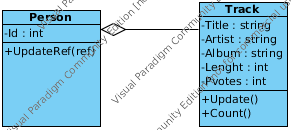
\includegraphics[width=0.5\linewidth]{Images/BackendDSv1.png}
  \caption{Data structure of the backend}
  \label{fig:backendDS}
\end{figure}
